\documentclass{style/CRPITStyle}
\usepackage{epsfig}   % Packages to use if you wish
\usepackage{lscape}   %
\usepackage[authoryear]{natbib}
\renewcommand{\cite}{\citep}
\pagestyle{empty}
\thispagestyle{empty}
\hyphenation{roddick}

\begin{document}

\title{Software Development Life Cycles: History and Future}
\author{David Barnett}
\affiliation{School of Engineering and Computer Science \\
Victoria University of Wellington, \\
PO Box 600, Wellington, 6140 \\
Email:~{\tt barentdavi@myvuw.ac.nz}}

\maketitle

% \begin{abstract}
%     % TODO
% \end{abstract}
\vspace{.1in}

\noindent {\em Keywords:} Software Process Models

\vspace{.1in}

% \section{Introduction}
% TODO
% thesis statement

\section{Importance of using process models}
% Q: describe the importance of using process models to guide software development
Fail to plan, is a plan to fail. 
As software has increased in complexity and scale of projects increase it
became more apparent that software should be managed and planned differently it was
described as a \emph{Software crisis} \cite{nato:1969}.
``We believe that the only way ahead lies through the steady development of the best existing 
techniques'' \cite{nato:1969} Gill's comments on how to move forward from the
\emph{Software Crisis} which describes a need for more of a engineering approach to software development.
One such endeavour is process modelling.
A process model is a model of how to setup a project with a set of tasks,
such as requirements acquisition or construction, of a similar nature that together form 
the scaffolding of a plan of how to approach to build a project.

\vspace{.1in} % are we allowed to do this?

By using the appropriate process model software development can be guided
through the many stages of creating software with an over-arching idea of how it
should be done. This can range from having static requirements and working
linearly through the development cycle to changing the requirements from week to
week. With the right processing model the software will have the correct tools
to handle what was expected to happen through out the process and give a guide
through the unexpected.

\vspace{.1in}
% TODO: this needs some reworking
Over the years many process models have been proposed and many variations have
been used and reported one. The process models that will be discussed in this
review is: Waterfall, V-Model, Spiral Model, Phased Development Model and
Extreme programming.

% --- 5 Model Section ---
% Q: provide a systematic review of process models that have been proposed so far,
% Q: compare and contract 5 selected distinct process models for software development
% Q: identify central themes that have been considered important for evolving process models
\section{Waterfall} % sequential
% theme: sequential
% strengths: requirements up front, easy
% Goals: a model of how to make successful large software
% Strengths: easy, clear steps and deliverables
% compare: ??
% contrast: ??
% Need a counter source, "Enough with Life cycle?"

The Waterfall model was proposed in 1970 by Dr. Winston Royce \cite{Waterfall:1970}.

\begin{figure}[htb]
\fbox{\parbox[b]{.99\linewidth}{
\vskip 0.5cm
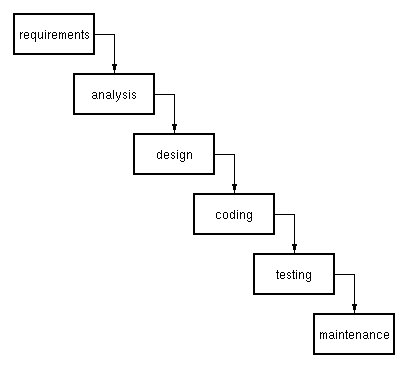
\includegraphics[width=0.45\textwidth]{figures/waterfall-model.png}
\vskip 0.5cm}}
\caption{\protect\label{xyz}  Waterfall Model}
\end{figure}

\section{V-Model} % sequential, testing
% theme:
% Goals: to extends the existing Waterfall to include testing
% compare: Waterfall's steps
% contrast: Has testing involved in the 

\section{Spiral Model} % sequential / Iterative, testing, risk
% theme:
% compare:
% contrast:

\section{Phased Development Model} % iterative, testing, risk
% theme:
% compare:
% contrast:

\section{Extreme Programming} % iterative, testing, risk
% theme:
% compare:
% contrast:

\section{Possible evolutions of process models}
% Q: try to forecast how current process models may evolve in the future


\bibliographystyle{agsm}
\bibliography{essay}

\end{document}

% ------- Example Area ------
% section example
% \section{Heading Level 1}
% \subsection{Heading Level 2}
% \subsubsection{Heading Level 3}

% figure example
% \begin{figure}[htb]
% \fbox{\parbox[b]{.99\linewidth}{
% \vskip 0.5cm
% \centerline{Figure Content}
% \vskip 0.5cm}}
% \caption{\protect\label{xyz}  Caption}
% \end{figure}

% ...as proved by \citet{Snodgrass87} and \citet{FPS96} and referred to in other works \cite{BenZvi82,Bentley86,AIS93} the process..., etc.

% list example
% \begin{enumerate}
% \item Not having the correct margins -- they are 0.8 inch all round.
% \item Not using A4 paper format when creating the pdf file.
% \end{enumerate}
% vim:set spell et sw=4 ts=4 tw=80:
